\section{Используемые технологии и аппаратная платформа}


\subsection{Язык программирования С++}

С++ является языком программирования общего назначения. Естественная для него область
применения - системное программирование, понимаемое в широком смысле этого слова. Кроме того,С++ успешно используется во многих областях приложения, далеко выходящих за указанные рамки.Реализации С++ теперь есть на всех машинах, начиная с самых скромных микрокомпьютеров - до самых больших супер-ЭВМ, и практически для всех операционных систем. Поэтому книга дает лишь описание собственно языка, не объясняя особенности конкретных реализаций, среды программирования или библиотек.

С++ - язык общего назначения и задуман для того, чтобы настоящие программисты получили
удовольствие от самого процесса программирования. За исключением второстепенных деталей он содержит язык С как подмножество. Язык С расширяется введением гибких и эффективных средств, предназначенных для построения новых типов. Программист структурирует свою задачу, определив новые типы, которые точно соответствуют понятиям предметной области задачи. Такой метод построения программы обычно называют абстракцией данных. Информация о типах содержится в некоторых объектах типов, определенных пользователем. С такими объектами можно работать надежно и просто даже в тех случаях, когда их тип нельзя установить на стадии трансляции. Программирование с использованием таких объектов обычно называют объектно-ориентированным. Если этот метод применяется правильно, то программы становятся короче и понятнее, а сопровождение их упрощается.

Ключевым понятием С++ является класс. Класс - это определяемый пользователем тип. Классы обеспечивают упрятывание данных, их инициализацию, неявное преобразование пользовательских типов, динамическое задание типов, контролируемое пользователем управление памятью и средства для перегрузки операций. В языке С++ концепции контроля типов и модульного построения программ реализованы более полно, чем в С. Кроме того, С++ содержит усовершенствования, прямо с классами не связанные: символические константы, функции-подстановки, стандартные значения параметров
функций, перегрузка имен функций, операции управления свободной памятью и ссылочный тип. В С++ сохранены все возможности С эффективной работы с основными объектами, отражающими аппаратную "реальность" (разряды, байты, слова, адреса и т.д.). Это позволяет достаточно эффективно реализовывать пользовательские типы.

Как язык, так и стандартные библиотеки С++ проектировались в расчете на переносимость. Имеющиеся реализации языка будут работать в большинстве систем, поддерживающих С. В программах на С++ можно использовать библиотеки С. Большинство служебных программ, рассчитанных на С, можно использовать и в С++.

Развитие языка С++ происходило на базе языка С, и, за небольшим исключением, С был сохранен в качестве подмножества C++. Базовый язык С был спроектирован таким образом, что имеется очень тесная связь между типами, операциями, операторами и объектами, с которыми непосредственно работает машина, т.е. числами, символами и адресами. За исключением операций new, delete и throw, а также проверяемого блока, для выполнения операторов и выражений С++ не требуется скрытой динамической аппаратной или программной поддержки.

В С++ используется та же (или даже более эффективная) последовательность команд для вызова функций и возврата из них, что и в С. Если даже эти довольно эффективные операции становятся слишком дорогими, то вызов функции может быть заменен подстановкой ее тела, причем сохраняется удобная функциональная запись безо всяких расходов на вызов функции.

Первоначально язык С задумывался как конкурент ассемблера, способный вытеснить его из основных и наиболее требовательных к ресурсам задач системного программирования. В проекте С++ были приняты меры, чтобы успехи С в этой области не оказались под угрозой. Различие между двумя языками прежде все состоит в степени внимания, уделяемого типам и структурам. Язык С выразителен и в то же время снисходителен по отношению к типам. Язык С++ еще более выразителен, но такой выразительности можно достичь лишь тогда, когда типам уделяют большое внимание. Когда типы объектов известны, транслятор правильно распознает такие выражения, в которых иначе программисту пришлось бы записывать операции с утомительными подробностями. Кроме того, знание типов позволяет транслятору обнаруживать такие ошибки, которые в противном случае были бы выявлены только при тестировании. Отметим, что само по себе использование строгой типизации языка для контроля параметров функции, защиты данных от незаконного доступа, определения новых типов и операций не влечет дополнительных расходов памяти и увеличения времени выполнения программы.

В проекте С++ особое внимание уделяется структурированию программы. Это вызвано увеличением размеров программ со времени появления С. Небольшую программу (скажем, не более 1000 строк) можно заставить из упрямства работать, нарушая все правила хорошего стиля программирования. Однако, действуя так, человек уже не сможет справиться с большой программой. Если у вашей программы в 10 000 строк плохая структура, то вы обнаружите, что новые ошибки появляются в ней так же быстро, как удаляются старые. С++ создавался с целью, чтобы большую программу можно было
структурировать таким образом, чтобы одному человеку не пришлось работать с текстом в 25000 строк. В настоящее время можно считать, что эта цель полностью достигнута.

Существуют, конечно, программы еще большего размера. Однако те из них, которые действительно используются, обычно можно разбить на несколько практически независимых частей, каждая из которых имеет значительно меньший упомянутого размер. Естественно, трудность написания и сопровождения программы определяется не только числом строк текста, но и сложностью предметной области. Так что приведенные здесь числа, которыми обосновывались наши соображения, не надо воспринимать слишком серьезно.

К сожалению, не всякую часть программы можно хорошо структурировать, сделать независимой от аппаратуры, достаточно понятной и т.д. В С++ есть средства, непосредственно и эффективно представляющие аппаратные возможности. Их использование позволяет избавиться от беспокойства о надежности и простоте понимания программы. Такие части программы можно скрывать, предоставляя надежный и простой интерфейс с ними.

Естественно, если С++ используется для большой программы, то это означает, что язык используют группы программистов. Полезную роль здесь сыграют свойственные языку модульность, гибкость и строго типизированные интерфейсы. В С++ есть такой же хороший набор средств для создания больших программ, как во многих языках. Но когда программа становится еще больше, проблемы по ее созданию и сопровождению перемещаются из области языка в более глобальную область программных средств и управления проектом \cite{StroustrupCpp}.


\subsection{Тулчейны}

Так исторически сложилось, что компиляторы не работают в изоляции. На практике пользователь вообще редко запускает компилятор напрямую. И gcc, и clang, и даже icc — это просто программы-оболочки (также говорят "драйверы"), которые запускают из-под себя не только компилятор, но и много что ещё. Конечно, пользователя интересует результат: превращение текста программы в исполняемый файл. Но именно для достижения такого результата одного только компилятора мало. Когда в обыденном языке мы говорим "компилятор GCC", мы обычно имеем в виду как раз ту самую программу-оболочку, под которой скрывается GNU Toolchain — громадный и разветвлённый набор компонентов и библиотек.

Если вы интересуетесь именно компилятором, то очень важно знать и понимать его место в тулчейне. И даже если рассматривать компилятор отдельно, он занимается не только оптимизациями. Поэтому не менее важно знать место оптимизатора в компиляторе.
Общий ландшафт вокруг компиляторов сформирован самыми разными инструментами разработки — ассемблерами, линкерами, отладчиками, профилировщиками. Конечно, мне не хватит места поговорить о них всех. То немногое, о чём я успею здесь рассказать, как мне кажется, важно знать не только если вы разрабатываете компиляторы, но даже если вы просто пользуетесь ими.

\begin{figure}[H]
	\centering
	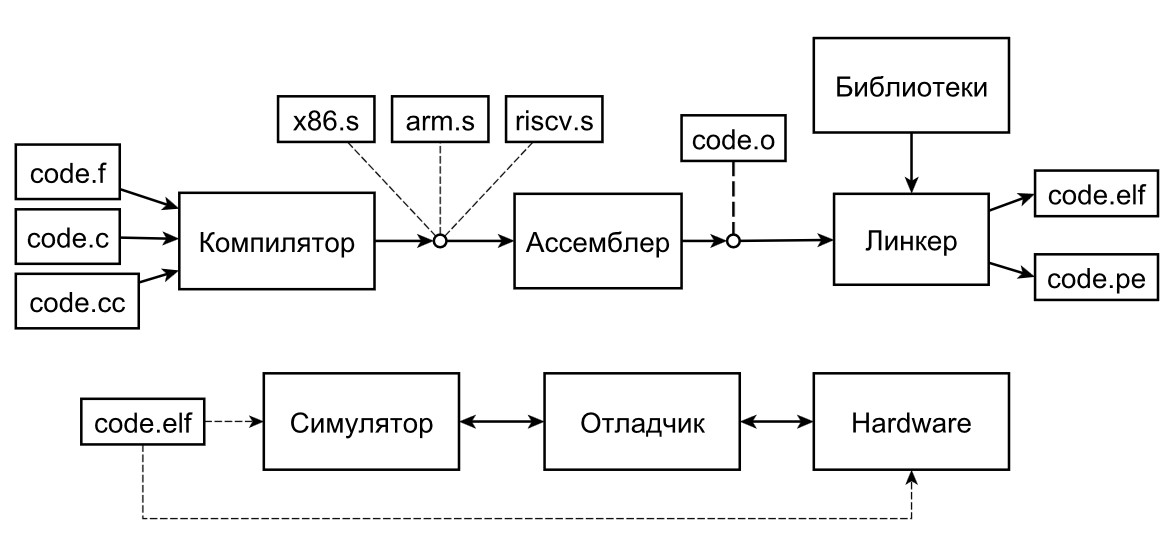
\includegraphics[scale=0.5]{tul.jpg}
	\caption{Упрощенная схема тулчейна}
	\label{fig:tulchain}
\end{figure}

Упрощённая схема тулчейна приведена на рисунке \ref{fig:tulchain}. Основными её частями являются компилятор, ассемблер и линкер. Кроме того, показано, что получившийся бинарник (binary file, слептовое выражение для файла, содержащего не текст, а двоичный код) можно отлаживать и запускать на железе или на симуляторе. Запуски на симуляторе могут быть полезны при кросс-компиляции, например, если вы на одной архитектуре компилируете код для исполнения на другой.

Итак, под общей крышей программы-драйвера в основном живут компилятор, ассемблер и линкер. Настало время посмотреть на эти основные части поближе.

Компилятор — это основа, главная и самая сложная часть тулчейна. Как можно судить по рисунку \ref{fig:tulchain} компилятор решает задачу, кажущуюся простой — он берёт программу на высокоуровневом языке и строит из неё ассемблерный код. 

Большинство компиляторов работают по правилу, известному как "as if rule" — они оптимизируют программу так, чтобы последовательность побочных эффектов, порождаемых её корректным исполнением, была такой же, как если бы программа выполнялась написавшим её программистом в уме. Ключевым в этом правиле является именно то, что оно закладывается только на корректное исполнение. Исполнение, приводящее к неопределённому поведению (например, к знаковому целочисленному переполнению), считается невозможным и оптимизатором не учитывается.

Конструктивно компилятор состоит из фронтенда (compiler frontend), который занимается построением промежуточного представления из исходного кода, а также из бэкенда (compiler backend), который занимается его оптимизациями и кодогенерацией. Англицизмы "фронтенд" и "бэкенд" неизбежны: во-первых, они укрепились в технической традиции и не только в компиляторах — свои фронтенды есть и в вебе, и в других областях (и там они значат другое); во-вторых, адекватные переводы являются громоздкими и скорее запутывают. Иногда оптимизации выделяют в "мидленд" (middle-end), оставляя в бэкенде только кодогенерацию, но в индустрии термин "мидленд" не распространён, и я буду объединять его с бэкендом, разделяя бэкенд на оптимизатор и кодогенератор.

Под словом "ассемблер" обычно понимается либо язык ассемблера для конкретной архитектуры, либо ассемблер как программа, которая транслирует программу на языке ассемблера в объектный код (object code). Объектным кодом называется специальное представление машинного кода, в котором инструкции уже закодированы, но который всё ещё предназначен не для исполнения, а для дальнейшей линковки (после которой он становится исполняемым кодом). В некоторых тулчейнах ассемблер как программа может быть (опционально) встроен в компилятор, и тогда объектный код порождает сразу компилятор.

Здесь может возникнуть сразу несколько вопросов.

Например, зачем вообще нужен язык ассемблера, если можно сразу порождать объектный код? Наличие отдельного языка ассемблера мотивировано, во-первых, тем, что дизассемблер читать и отлаживать гораздо проще, чем бинарный код. Отладка по ассемблерному коду — это нормальный сценарий для отладки сложных проблем, плохо проявляющихся в отладочных сборках. Во-вторых, набор инструкций для каждой архитектуры обычно куда больше, чем всё, что может породить компилятор. Существуют специальные инструкции для работы с системными регистрами, и писать хотя бы небольшие программы на языке ассемблера в некоторых случаях приходится (например, при написании операционных систем).

Ещё один возможный вопрос: зачем нужен объектный код, почему бы сразу не порождать исполняемый файл, минуя промежуточные фазы? Здесь мотивация ещё проще. В большинстве известных мне языков программирования предусмотрена в том или ином виде раздельная трансляция. Как минимум она нужна для того, чтобы получить возможность иметь предварительно скомпилированный библиотечный код. Для такого кода необходим механизм, который позволял бы сохранять информацию для разрешения межмодульных вызовов. Одновременно этот механизм не слишком нужен в итоговом исполняемом файле, где все кросс-модульные зависимости уже разрешены. Это и мотивирует наличие объектного кода.

Статическая линковка запускается после ассемблирования. В самом простом случае можно просто отдать линкеру (например, GNU ld) ваши объектные файлы и стандартные библиотеки. Однако пути к стандартным библиотекам обычно сильно зависят от опций сборки. Например, у вас будет разная стандартная библиотека для 32-битного и 64-битного кода, а также разная для разных ABI в тех архитектурах, где это применимо. Поэтому обычно пути к стандартным библиотекам формирует драйвер компилятора на основании известных ему (иногда неочевидных) соображений. Эти пути всегда можно подсмотреть, но никогда не рекомендуется задавать явно вручную \cite{Vladimirov2024}.

\subsection{Генератор систем сборки CMake}

Если вам когда-либо приходилось поддерживать процесс сборки и установки программного пакета, вас наверняка заинтересует CMake. CMake — это генератор систем сборки с открытым исходным кодом, который позволяет разработчикам задавать параметры сборки в простом, переносимом текстовом формате. Этот файл затем используется CMake для генерации проектных файлов под нативные инструменты сборки, включая интегрированные среды разработки (IDE), такие как Microsoft Visual Studio или Apple Xcode, а также UNIX, Linux, NMake и Ninja. CMake упрощает сложные аспекты сборки программного обеспечения, такие как кроссплатформенная сборка, анализ системы и настройка под пользовательские требования, предоставляя удобные средства для адаптации сборки под сложные аппаратные и программные системы.

С 1999 года CMake активно развивается и достиг уровня, когда он стал проверенным решением для широкого круга задач сборки. Разработка CMake началась в рамках проекта Insight Toolkit (ITK), финансируемого Национальной медицинской библиотекой США. ITK — это крупный программный проект, который должен работать на множестве платформ и взаимодействовать с другими программными пакетами. Чтобы обеспечить это, потребовался мощный, но простой в использовании инструмент сборки. Опираясь на опыт работы с системами сборки для больших проектов, разработчики создали CMake, учитывая эти потребности. С тех пор популярность CMake неуклонно растёт, и многие проекты и разработчики выбирают его за простоту и гибкость. Наиболее яркий пример — успешное внедрение CMake в качестве системы сборки K Desktop Environment (KDE), одного из крупнейших проектов с открытым исходным кодом.

Для любого проекта, особенно кроссплатформенного, необходима единая система сборки. Многие проекты, не использующие CMake, поставляются как с Makefile (или Makefile.in) для UNIX, так и с рабочей областью Microsoft Visual Studio. Это вынуждает разработчиков постоянно поддерживать обе системы сборки в актуальном и согласованном состоянии. Добавление поддержки других систем, например Xcode, требует ещё большего количества кастомных файлов, усугубляя проблему. Ситуация становится ещё сложнее, если нужно поддерживать опциональные компоненты, такие как подключение JPEG-поддержки при наличии libjpeg в системе. CMake решает эту проблему, объединяя все эти операции в одном простом и понятном формате файла.

CMake также включает поддержку тестирования программного обеспечения через CTest. Часть процесса тестирования включает сборку, возможную установку и определение того, какие компоненты программного обеспечения подходят для текущей системы. Это делает CTest логичным расширением CMake, поскольку он уже содержит большую часть этой информации. Аналогичным образом, CMake включает CPack — инструмент для кросс-платформенного распространения программного обеспечения. Он предоставляет универсальный способ создания нативных установщиков, используя популярные форматы, такие как WiX, RPM, Cygwin и PackageMaker.

Если над проектом работает несколько разработчиков или он предназначен для нескольких целевых платформ, сборка будет выполняться на разных компьютерах. Учитывая разнообразие установленного ПО и пользовательских настроек современных систем, даже две машины с одной ОС могут иметь различия. CMake предоставляет множество преимуществ для одноплатформенных, но многомашинных сред разработки, включая:
\begin{itemize}
	\item Автоматический поиск зависимостей;
	\item Отдельная директория сборки;
	\item Генерация исходного кода;
	\item Выбор компонентов;
	\item Генерация проектов;
	\item Параллельная сборка.
\end{itemize}

CMake продолжает поддерживать новые инструменты сборки по мере их появления. Он быстро добавляет совместимость с новыми версиями Microsoft Visual Studio и Apple Xcode. Кроме того, в CMake была добавлена поддержка Ninja — современного инструмента сборки от Google. Благодаря CMake, после написания конфигурационных файлов вы автоматически получаете поддержку новых компиляторов и систем сборки, так как она встроена в новые версии CMake и не зависит от вашего дистрибутива. CMake также обеспечивает кросс-компиляцию для других операционных систем или встраиваемых устройств. Большинство команд в CMake корректно обрабатывают различия между хост-системой и целевой платформой при кросс-компиляции.

\subsection{Система контроля версий Git}

Система контроля версий — это система, записывающая изменения в файл или набор файлов в течение времени и позволяющая вернуться позже к определённой версии.

Многие люди в качестве метода контроля версий применяют копирование файлов в
отдельный каталог. Данный подход очень распространён из-за его простоты, однако он
невероятно сильно подвержен появлению ошибок. Можно легко забыть в каком каталоге
вы находитесь и случайно изменить не тот файл или скопировать не те файлы, которые вы
хотели.

Как и многие вещи в жизни, Git начинался с капелькой творческого хаоса и бурных споров.

Ядро Linux — это достаточно большой проект с открытым исходным кодом. Большую часть
времени разработки ядра Linux (1991–2002 гг.) изменения передавались между
разработчиками в виде патчей и архивов. В 2002 году проект ядра Linux начал использовать
проприетарную децентрализованную систему контроля версий BitKeeper.

В 2005 году отношения между сообществом разработчиков ядра Linux и коммерческой
компанией, которая разрабатывала BitKeeper, прекратились, и бесплатное использование
утилиты стало невозможным. Это сподвигло сообщество разработчиков ядра Linux (а в
частности Линуса Торвальдса — создателя Linux) разработать свою собственную утилиту,
учитывая уроки, полученные при работе с BitKeeper. Некоторыми целями, которые
преследовала новая система, были:
\begin{itemize}
	\item Скорость;
	\item Простая архитектура;
	\item Хорошая поддержка нелинейной разработки (тысячи параллельных веток);
	\item Полная децентрализация;
	\item Возможность эффективного управления большими проектами, такими как ядро Linux;
\end{itemize}
С момента своего появления в 2005 году, Git развился в простую в использовании систему, сохранив при этом свои изначальные качества. Он удивительно быстр, эффективен в работе с большими проектами и имеет великолепную систему веток для нелинейной разработки.

Основное отличие Git от любой другой системы контроля версий (включая Subversion и её
собратьев) — это подход к работе со своими данными. Концептуально, большинство других
систем хранят информацию в виде списка изменений в файлах. Эти системы (CVS,
Subversion, Perforce, Bazaar и т. д.) представляют хранимую информацию в виде набора
файлов и изменений, сделанных в каждом файле, по времени (обычно это называют
контролем версий, основанным на различиях).

Git не хранит и не обрабатывает данные таким способом. Вместо этого, подход Git к
хранению данных больше похож на набор снимков миниатюрной файловой системы.
Каждый раз, когда вы делаете коммит, то есть сохраняете состояние своего проекта в Git, система запоминает, как выглядит каждый файл в этот момент, и сохраняет ссылку на этот снимок. Для увеличения эффективности, если файлы не были изменены, Git не запоминает эти файлы вновь, а только создаёт ссылку на предыдущую версию идентичного файла, который уже сохранён. Git представляет свои данные как, скажем, поток снимков.

Это очень важное различие между Git и почти любой другой системой контроля версий. Git переосмысливает практически все аспекты контроля версий, которые были скопированы
из предыдущего поколения большинством других систем. Это делает Git больше похожим
на миниатюрную файловую систему с удивительно мощными утилитами, надстроенными
над ней, нежели просто на VCS. Когда мы будем рассматривать управление ветками в главе Ветвление в Git, мы увидим, какие преимущества вносит такой подход к работе с данными в Git.

Для работы большинства операций в Git достаточно локальных файлов и ресурсов —  в основном, системе не нужна никакая информация с других компьютеров в вашей сети.
Если вы привыкли к централизованным системам контроля версий, где большинство
операций страдают от задержек из-за работы с сетью, то этот аспект Git заставит вас думать, что боги скорости наделили Git несказанной мощью. Так как вся история проекта хранится прямо на вашем локальном диске, большинство операций кажутся чуть ли не мгновенными.

Для примера, чтобы посмотреть историю проекта, Git не нужно соединяться с сервером для её получения и отображения — система просто считывает данные напрямую из локальной базы данных. Это означает, что вы увидите историю проекта практически моментально. Если вам необходимо посмотреть изменения, сделанные между текущей версией файла и версией, созданной месяц назад, Git может найти файл месячной давности и локально вычислить изменения, вместо того, чтобы запрашивать удалённый сервер выполнить эту операцию, либо вместо получения старой версии файла с сервера и выполнения операции локально.

Это также означает, что есть лишь небольшое количество действий, которые вы не сможете выполнить, если вы находитесь оффлайн или не имеете доступа к VPN в данный момент. Если вы в самолёте или в поезде и хотите немного поработать, вы сможете создавать коммиты без каких-либо проблем (в вашу локальную копию, помните?): когда будет возможность подключиться к сети, все изменения можно будет синхронизировать. Если вы ушли домой и не можете подключиться через VPN, вы всё равно сможете работать.
Добиться такого же поведения во многих других системах либо очень сложно, либо вовсе
невозможно. В Perforce, для примера, если вы не подключены к серверу, вам не удастся
сделать многого; в Subversion и CVS вы можете редактировать файлы, но вы не сможете
сохранить изменения в базу данных (потому что вы не подключены к БД). Всё это может
показаться не таким уж и значимым, но вы удивитесь, какое большое значение это может
иметь.

В Git для всего вычисляется хеш-сумма, и только потом происходит сохранение. В
дальнейшем обращение к сохранённым объектам происходит по этой хеш-сумме. Это
значит, что невозможно изменить содержимое файла или каталога так, чтобы Git не узнал
об этом. Данная функциональность встроена в Git на низком уровне и является
неотъемлемой частью его философии. Вы не потеряете информацию во время её передачи и
не получите повреждённый файл без ведома Git \cite{ProGit}.

\subsection{Одноплатный компьютер Raspberry Pi}

\newpage
